\section{Experiments}
\label{sec:experiment}

% order of description:
% - cold playlists
% - cold songs
% - cold users

In this section, we describe experiments that empirically evaluate the proposed method and a number of 
well known baseline approaches in the three cold-start settings described in Section~\ref{sec:problem}.


\subsection{Dataset}
We make use of two publicly available playlist datasets: the 30Music~\cite{30music2015} and AotM-2011~\cite{mcfee2012hypergraph} dataset.
The Million Song Dataset~\cite{msd2011} serves as an underlying dataset where songs in all playlists are intersected.
It also provides a few song features which will be described later in this section.

\begin{table}[hbt]
\centering
\caption{Music playlist dataset}
\label{tab:stats_pldata}
\resizebox{\linewidth}{!}{
\setlength\tabcolsep{3pt}
\begin{tabular}{lrcrrccc}
\toprule
Dataset   & Songs   & Playlists & Users   & Artists & Songs/Playlist & Playlists/User & Songs/Artist \\
\midrule                                                                                             
30Music   & 45,468  & 17,457    & 8,070   & 9,981   & 16.3           & 2.2            & 28.6 \\
AotM-2011 & 114,428 & 84,710    & 14,182  & 15,698  & 10.1           & 6.0            & 53.8 \\
\bottomrule
\end{tabular}
}
\end{table}


{\bf Million Song Dataset} (MSD) is a collection of one million songs, where each song is described by its metadata 
(\eg song title, artist name, year of release) and a number of precomputed audio features from the Echo Nest\footnote{http://the.echonest.com}.
%It also provides acoustic features computed from a sample section of audio file of each song. % more description

{\bf 30Music Dataset} is a collection of listening events and playlists retrieved from Last.fm\footnote{https://www.last.fm}.
We first intersect the playlists data with songs in the MSD, 
%leveraging the Last.fm dataset~\cite{lastfmdataset} which matched songs from Last.fm with those in the MSD, 
then filter out playlists with less than 5 songs.
This results in about 17K playlists over 45K songs from 8K users.

{\bf AotM-2011 Dataset} is a collection of playlists shared by Art of the Mix\footnote{http://www.artofthemix.org} 
users during the period from 1998 to 2011. Songs in playlists have been matched to those in the MSD.
We filtered out playlists with less than 5 songs, which results in roughly 84K playlists over 114K songs from 14K users.
%
Table~\ref{tab:stats_pldata} summarises the %two 
playlist datasets used in this work.



\begin{table*}[!t]
    \centering
    \begin{minipage}{.35\textwidth}
        \centering
        \caption{Dataset for \emph{cold songs}}
        \label{tab:stats0}
        \resizebox{.9\textwidth}{!}{
        \begin{tabular}{lrrcrr}
        \toprule
        \multirow{2}{*}{Dataset}  & \multicolumn{2}{c}{Songs} && \multicolumn{2}{c}{Playlists} \\ \cmidrule{2-3} \cmidrule{5-6}
                                  & Train & Test && Train & Test \\
        \midrule
        30Music   & 40,468  & 5,000  && 17,342  & 8,215 \\
        AotM-2011 & 104,428 & 10,000 && 84,646  & 19,504 \\
        \bottomrule
        \end{tabular}
        }
    \end{minipage}%
    \begin{minipage}{0.33\textwidth}
        \centering
        \caption{Dataset for \emph{cold playlists}}
        \label{tab:stats1}
        \resizebox{.9\textwidth}{!}{
        \begin{tabular}{lrrcrr}
        \toprule
        \multirow{2}{*}{Dataset}  & \multicolumn{2}{c}{Playlists} && \multicolumn{2}{c}{Users} \\ \cmidrule{2-3} \cmidrule{5-6}
                                  & Train & Test && Train & Test \\
        \midrule
        30Music   & 15,262 & 2,195 &&  8,070 & 1,644 \\
        AotM-2011 & 75,477 & 9,233 && 14,182 & 2,722 \\
        \bottomrule
        \end{tabular}
        }
    \end{minipage}%
    \begin{minipage}{.33\textwidth}
        \centering
        \caption{Dataset for \emph{cold users}}
        \label{tab:stats2}
        \resizebox{.9\textwidth}{!}{
        \begin{tabular}{lrrcrr}
        \toprule
        \multirow{2}{*}{Dataset}  & \multicolumn{2}{c}{Playlists} && \multicolumn{2}{c}{Users} \\ \cmidrule{2-3} \cmidrule{5-6}
                                  & Train & Test && Train & Test \\
        \midrule
        30Music   & 14,067 & 3,390 && 5,649 & 2,421 \\
        AotM-2011 & 76,450 & 8,260 && 9,928 & 4,254 \\
        \bottomrule
        \end{tabular}
        }
    \end{minipage}
\end{table*}


\subsection{Experimental setup}

We describe how playlists in the two datasets are split into training and test set for the three cold-start settings,
and the features of songs used to learn the multitask objective, as well as baseline approaches and evaluation metrics.

\subsubsection{Dataset split}
To empirically evaluate the performance of recommending new songs to extend existing playlists (\ie the \emph{cold songs} setting),
we hold 5K of the latest released songs in the 30Music dataset. 
This results in about 8K playlists with songs in both the training and test set.
In the AotM-2011 dataset where more songs are available, we hold 10K of the latest released songs.
This leads to about 19K playlists with songs in both the training and test set.
We remove playlists where all songs have been held for test. %are removed from both the training and test set.
Table~\ref{tab:stats0} summarises the statistics of this training/test split.

For the task of recommending songs to form new playlists for existing users (\ie the \emph{cold playlists} setting),
%To empirically evaluate the performance of our proposed recommendation approaches for existing users,
we hold playlists from about 20\% users in both datasets for test, and all other playlists are used for training.
The test set is formed by sampling playlists where each song has been included in at least five playlists among the whole dataset.
We also make sure each song in the test set also appears in the training set,
and all users in the test set also have a number of playlists in the training set.
This results in a test set with about 2.1K playlists from 1.6K users in 30Music dataset,
and a test set with about 9.2K playlists from 2.7K users in AotM-2011 dataset.
The statistics of this training/test split are shown in Table~\ref{tab:stats1}.

To evaluate the task of recommending songs for new users to form playlists (\ie the \emph{cold users} setting),
%To evaluate the performance of music recommendation approaches for new users,
we sampled 30\% of all users and hold all their playlists in both datasets.
Similarly, we require songs in the test set also exist in the training set,
a user will thus not be included in the test set if holding all of her playlists breaks this requirement.
This results in a test set with about 3.4K playlists from 2.4K users in 30Music dataset,
and a test set with about 8.2K playlists from 4.2K users in AotM-2011 dataset.
Table~\ref{tab:stats2} describes the statistics of this training/test split.


\subsubsection{Features}
% of songs used in the experiments include metadata, audio data, genre and artist information, as well as song and 
Song metadata, audio data, genre and artist information, as well as song and 
artist popularity (\ie the number of occurrences of all songs from the artist in training set)
are encoded as features.
%
The metadata of songs (\eg duration, year of release) and audio features (\eg loudness, mode, tempo) are provided by the MSD.
We use genre data from the Top-MAGD genre dataset~\cite{schindler2012facilitating}
and tagtraum genre annotations for the MSD~\cite{schreiber2015improving} via one-hot encoding.
If the genre data of a song is not available, we apply the mean imputation using genre counts of other songs in the training set.
To encode artist information as features,
we trained a word2vec\footnote{https://github.com/dav/word2vec} model using sequences of artist identifiers in playlists.

We assume no popularity information is available for newly released songs,
thus song popularity is used as a feature only in the \emph{cold playlists} and \emph{cold users} settings.
%In the task of recommending new songs to extend existing playlists (setting (i)), where song popularity is not available,
%we use artist popularity (we use the number of occurrences of all songs from a artist in training playlists as a proxy of her popularity).
Finally, we add a constant feature (with value $1$) for each song to account for bias.


\begin{figure*}[!t]
    \centering
    \begin{minipage}{.32\textwidth}
        \centering
        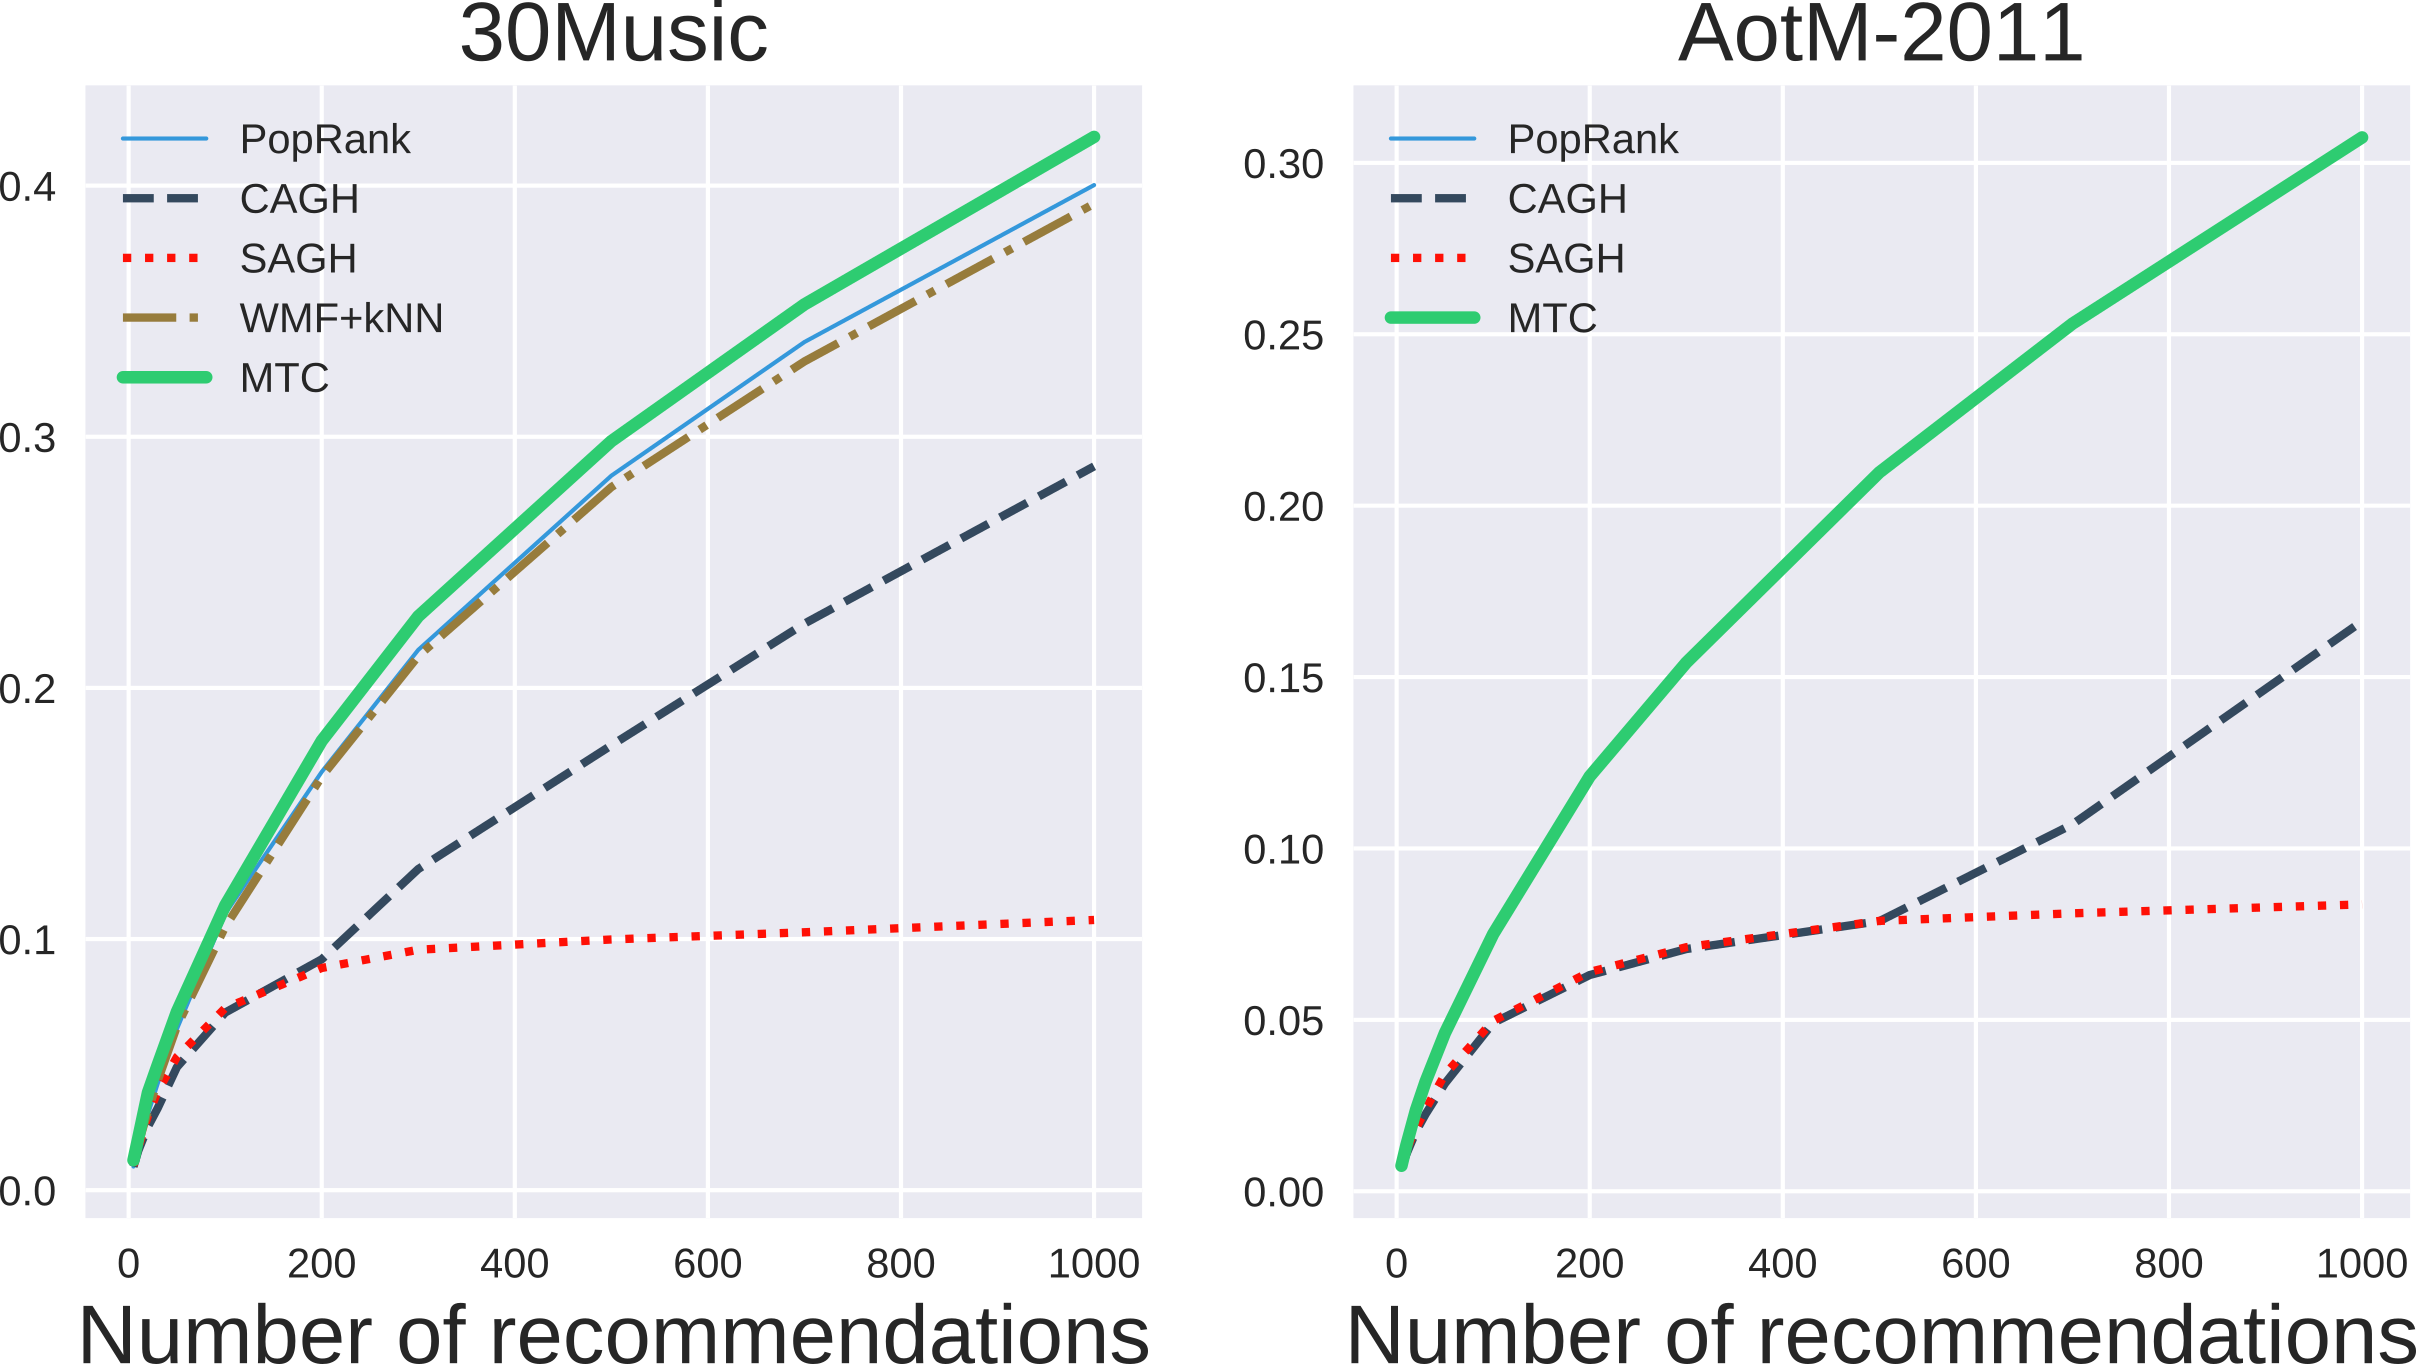
\includegraphics[width=.96\linewidth]{fig/hr4.png}
        \caption{Hit rates for {\it cold users}}
        \label{fig:hr4}
    \end{minipage}\hspace{11pt}%
    \begin{minipage}{0.32\textwidth}
        \centering
        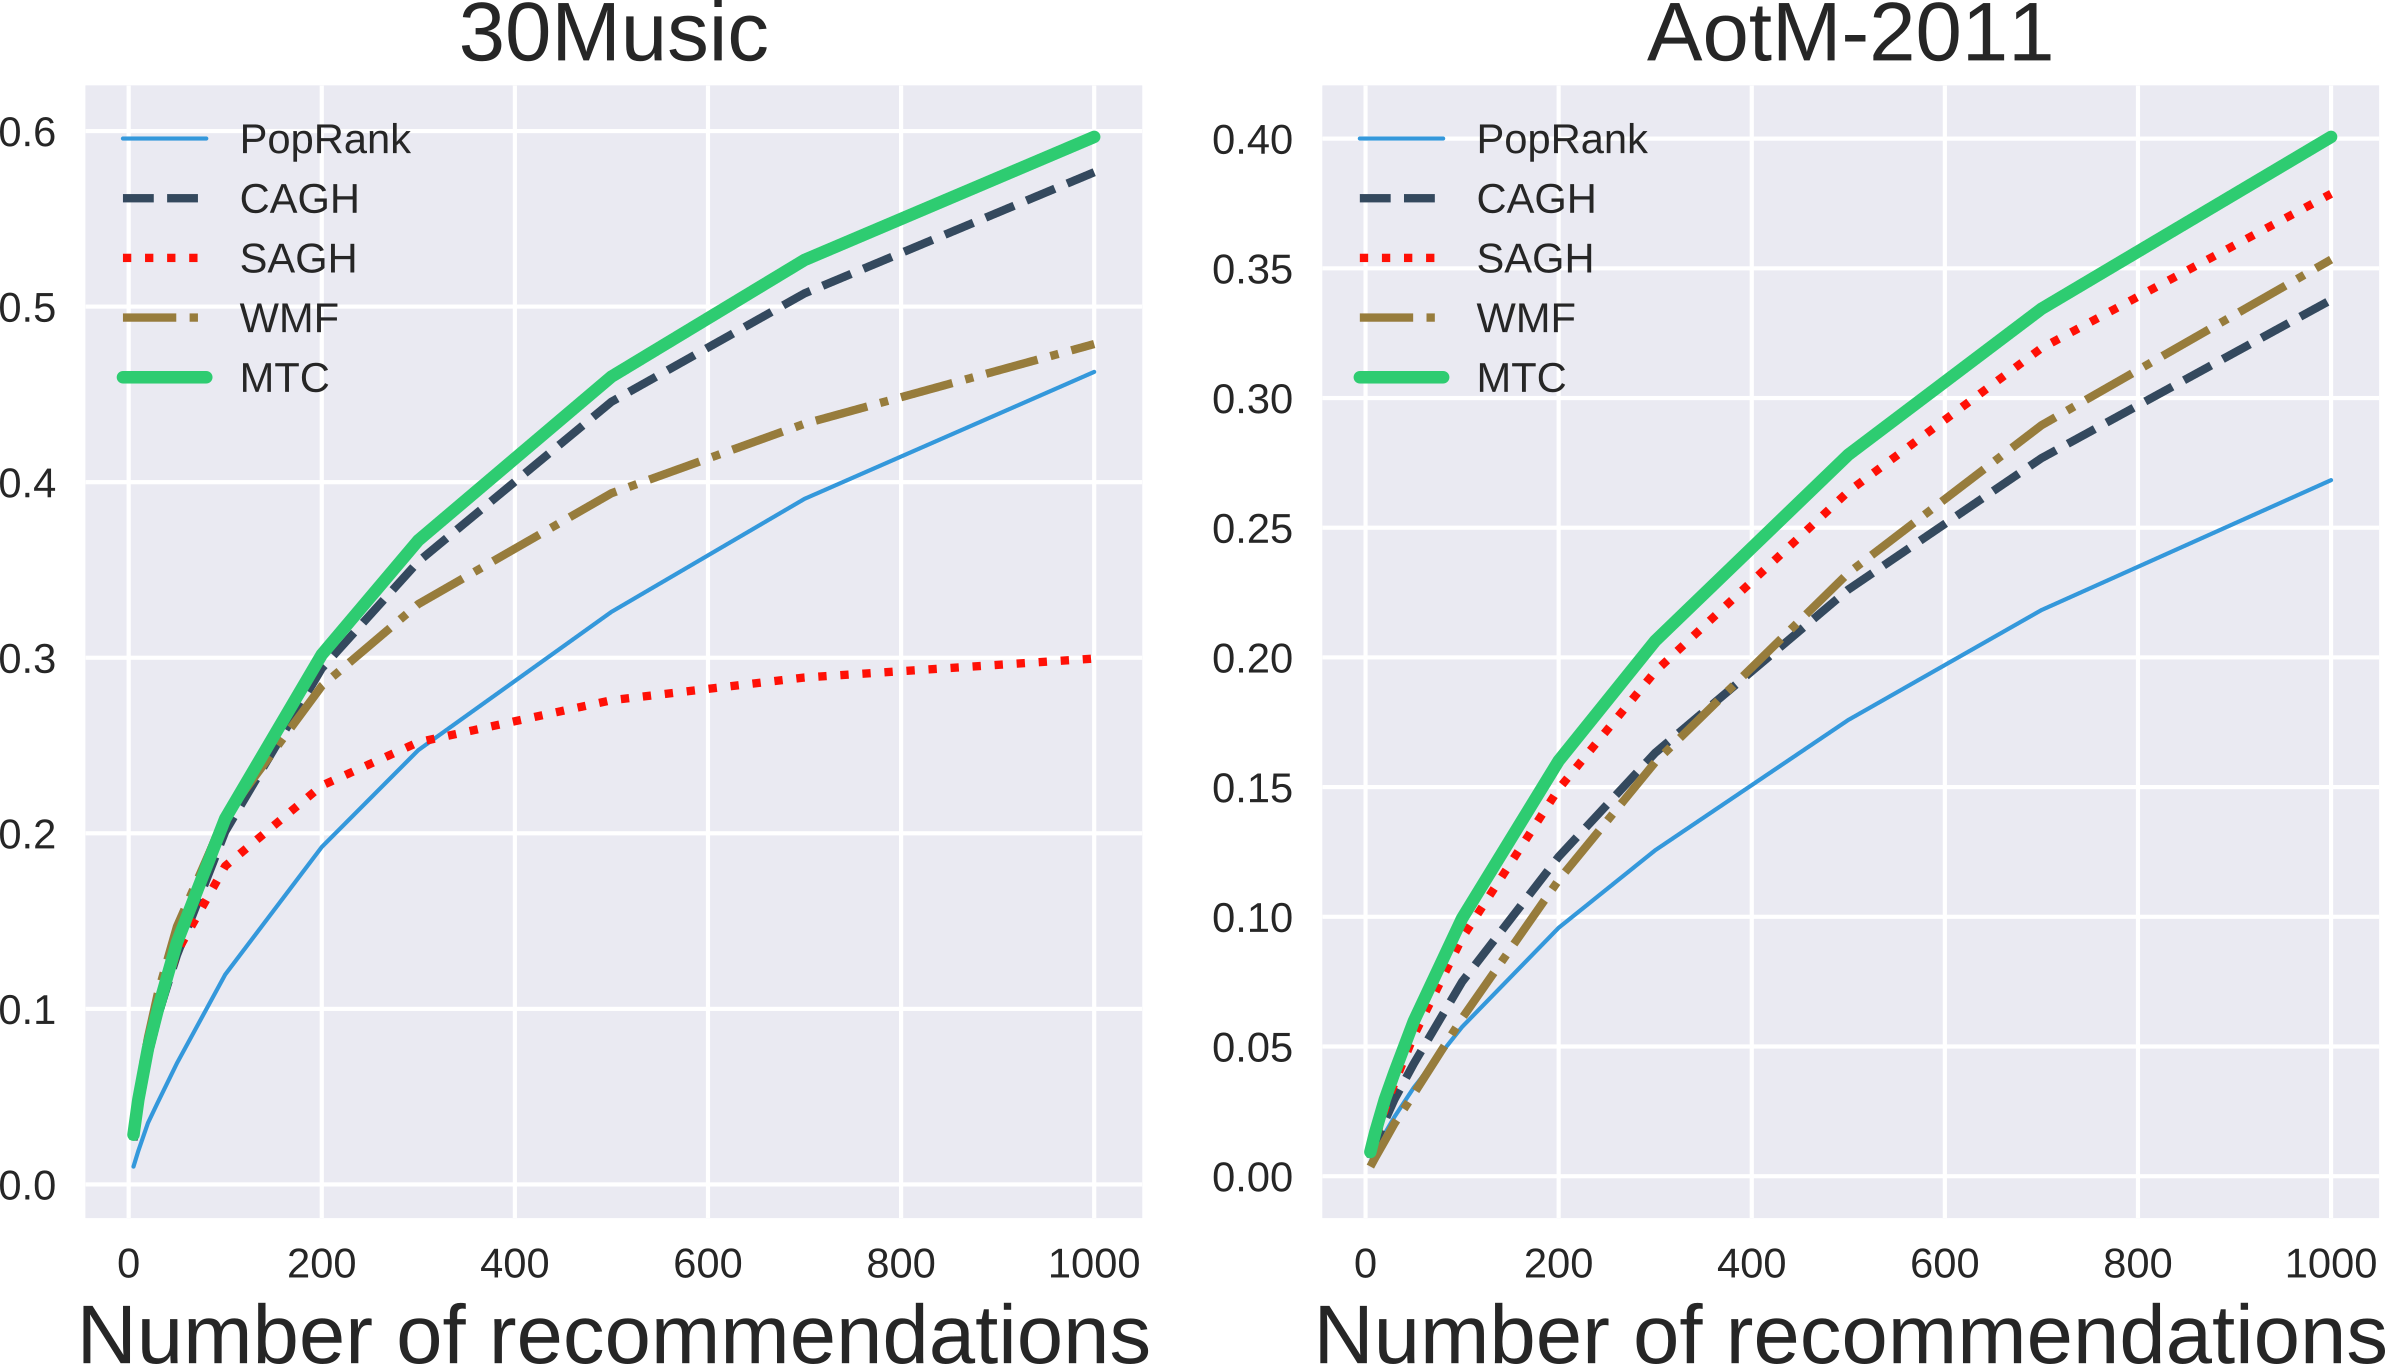
\includegraphics[width=.96\linewidth]{fig/hr3.png}
        \caption{Hit rates for {\it cold playlists}}
        \label{fig:hr3}
    \end{minipage}\hspace{8pt}%
    \begin{minipage}{0.32\textwidth}
        \centering
        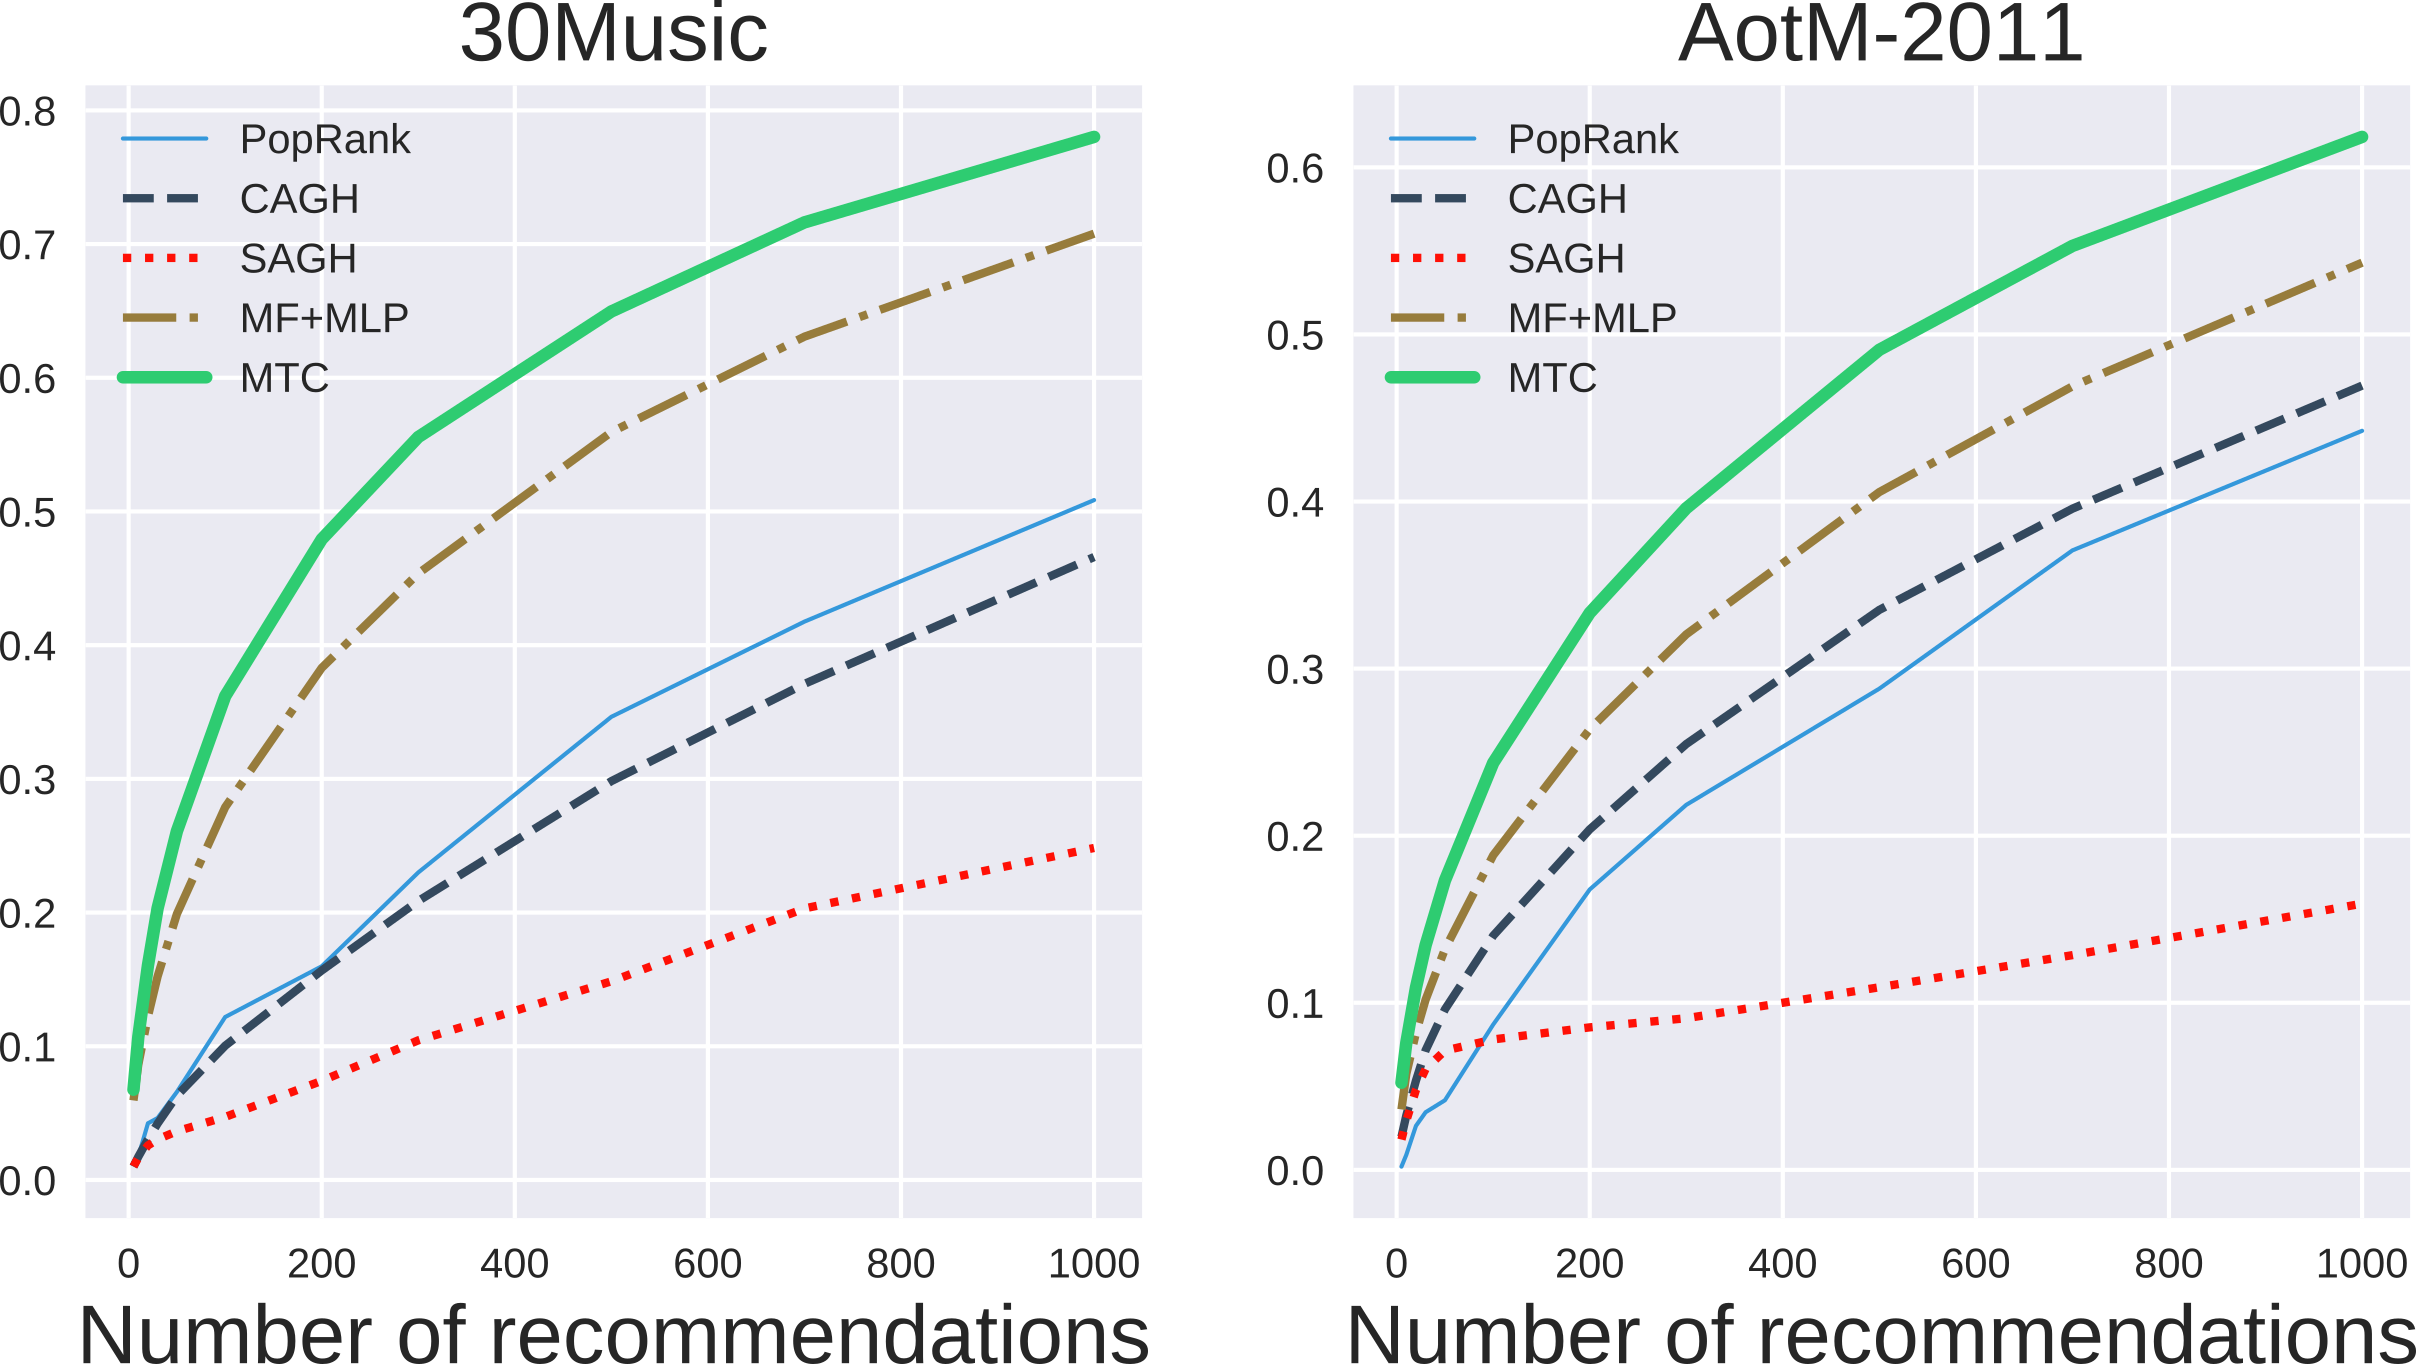
\includegraphics[width=\linewidth]{fig/hr1.png}
        \caption{Hit rates for {\it cold songs}}
        \label{fig:hr1}
    \end{minipage}
\end{figure*}


\subsubsection{Baselines}
We compare the performance of our proposed approach (\ie MTC) % (referred as {\it Multitask Classification}) 
with a number of baseline methods in the three cold-start settings:
%for the task of recommending music to form playlists:
\begin{itemize}
\item The {\it Popularity Ranking} (PopRank) method scores a song using only its popularity in the training set.
      In the \emph{cold songs} setting where song popularity is not available, 
      %we score a song using the popularity of the corresponding artist.
      a song is scored by the popularity of the corresponding artist.
\item The {\it Same Artists - Greatest Hits} (SAGH)~\cite{mcfee2012million} method scores a song
      by its popularity if the artist of the song has appeared in the given user's playlists (in training set);
      otherwise the song is scored zero.
      In the {\it cold songs} setting, this method considers only songs from artists appeared in the given playlist,
      and score them using the corresponding artist popularity.
%      Similarly, we replace song popularity with artist popularity in the \emph{cold songs} setting.
\item The {\it Collocated Artists - Greatest Hits} (CAGH)~\cite{bonnin2013evaluating} method is a variant of SAGH.
      It scores a song using its popularity, but weighted by the frequency of the collocation between the artist of the song
      and artists appeared in the given user's playlists (in training set).
      In the \emph{cold users} setting, we use the 10 most popular artists instead of artists in the user's listening history.
      The \emph{cold songs} setting is addressed in the same way as in SAGH.
%      as required by this method.
%\item The {\it Logistic Regression} baseline is specific for the \emph{cold songs} setting, where we independently learn 
%      a logistic regression classifier for each playlist, which is used to classify whether we should add each new song to 
%      this playlist\footnote{This method is also known as binary relevance in multi-label classification.}.
\item The three variants of Matrix Factorisation (MF), which first learn latent representations of songs, playlists or users
      through MF, then score each song by the dot product of the song and the corresponding playlist or user latent factors.
      Recommendations are made as per our method described in Section~\ref{sec:method}.
      In the \emph{cold songs} setting, latent representations of songs/playlists are learnt by factorising the song-playlist matrix  
      To obtain the representations of new songs, we learn a two-layer neural network (multilayer perceptron, MLP) to map song 
      content features to the corresponding latent representations~\cite{Gantner:2010,van2013deep}, and call this method MF+MLP. 
      In the \emph{cold playlists} setting, we factorise the song-user play-count matrix using the weighted matrix factorisation (WMF) 
      algorithm~\cite{hu2008collaborative,van2013deep} to learn the latent representations of songs and users.
      Similarly, latent representations of songs and users are learned using WMF in the \emph{cold users} setting, however, the latent 
      factor of a new user is approximated by the mean factors of the $k$ nearest neighbours (in terms of cosine similarity of user 
      attributes\footnote{User attributes include age, gender, country of the user, the number of playlists from her account, as well as 
      her total play counts and subscription type, these attributes are only available in the 30Music dataset. We choose $k=100$.}) 
      in training set, and we refer this method as WMF+kNN.
\end{itemize}




\subsubsection{Evaluation}
We evaluate the performance of all approaches using two accuracy metrics that have been adopted 
in playlist recommendation tasks:
HitRate@K~\cite{hariri2012context} and Area under the ROC curve (AUC)~\cite{manning2008introIR}.
%In addition to these accuracy related metrics, 
We further adopt two beyond-accuracy metrics, \ie
Novelty~\cite{zhang2012auralist,schedl2017} and Spread~\cite{kluver2014evaluating},
which are specifically tailored to recommender systems.
Unlike the accuracy metrics, where higher values indicate better performance,
\emph{moderate} values of Novelty and Spread are usually preferable~\cite{kluver2014evaluating,schedl2017}.
%
%R-Precision (RPREC) is the number of correctly recommended songs in the top-$n$ recommendation over $n$,
%where $n$ is the number of songs in the ground truth playlist.
%It is one of several metrics used to evaluate performance on playlist continuation tasks
%in the ACM RecSys Challenge 2018\footnote{https://recsys-challenge.spotify.com/rules}.

HitRate@K (or Recall@K) is the number of correctly recommended songs amongst the top-$K$ recommendations over
%where $K$ is the number of recommendations, and $L$ is 
the number of songs in the ground truth playlist. %\footnote{This metric is also known as Recall@K~\cite{schedl2017}.}.
It has been employed to evaluate several playlist generation and next song recommendation
methods~\cite{hariri2012context,bonnin2013evaluating,bonnin2015automated,jannach2015beyond}.

The area under the ROC curve (AUC) is widely used in measuring performance of classifiers,
it has also been used for evaluating performance of playlist generation method when the task
is cast as a (sequence of) classification problems~\cite{ben2017groove}.

Useful recommendations need to include previously unknown items~\cite{herlocker2004evaluating,zhang2012auralist}, 
and this ability can be measured by Novelty,
$$
\text{Novelty@K} = \frac{1}{U} \sum_{u=1}^U \frac{1}{|P_u|} \sum_{m \in S_K} \frac{-\log_2 pop_m}{K},
$$
where $S_K$ is the set of top-K recommendations and $pop_m$ is the popularity of song $m$.
Intuitively, the more popular a song is, an average user is more likely to be familiar with it,
therefore less novel to this user.

Spread is defined as the entropy of the distribution of all possible songs to recommend,
$$
\text{Spread} = -\sum_{m=1}^M P(m) \log P(m),
$$
where $P(m)$ denotes the probability of song $m$ being recommended,
which is computed from the scores of all possible songs using the softmax function.
Spread is used to measure the ability of an algorithm to spread its attention across all possible songs.


\subsection{Results and discussion}

% we compare the performance of our proposed approach with several other baseline approaches.
% we first analyse the accuracy related measures and look at measures that beyond accuracy.

%\begin{table*}[!t]
    \centering
    \begin{minipage}{.333\textwidth}
        \centering
        \caption{Accuracy for \emph{cold songs}}
        \label{tab:acc1}
        \resizebox{.97\textwidth}{!}{
        \setlength\tabcolsep{4pt}
        \begin{tabular}{l*{4}{c}*{4}{c}}
        \toprule
        \multirow{2}{*}{Method}      & \multicolumn{2}{c}{30Music} && \multicolumn{2}{c}{AotM-2011} \\ \cmidrule{2-3} \cmidrule{5-6}
                                     & HR@100 \% & AUC \% && HR@100 \% & AUC \% \\
        \midrule
        PopRank &         12.2 & 70.9 &&          8.7 & 76.5 \\
        CAGH    &         10.0 & 68.0 &&         14.0 & 77.4 \\
        SAGH    &          4.7 & 51.5 &&          7.8 & 53.6 \\
        MF+MLP  &         27.9 & 81.4 &&         18.8 & 80.8 \\
        MTC     &         {\bf 36.2} & {\bf 86.6} &&         {\bf 24.4} & {\bf 84.3} \\
        \bottomrule
        \end{tabular}
        }
    \end{minipage}%
    \begin{minipage}{0.332\textwidth}
        \centering
        \caption{Accuracy for \emph{cold playlists}}
        \label{tab:acc3}
        \resizebox{.96\textwidth}{!}{
        \setlength\tabcolsep{4pt}
        \begin{tabular}{l*{4}{c}*{4}{c}}
        \toprule
        \multirow{2}{*}{Method}      & \multicolumn{2}{c}{30Music} && \multicolumn{2}{c}{AotM-2011} \\ \cmidrule{2-3} \cmidrule{5-6}
                                     & HR@100 \% & AUC \% && HR@100 \% & AUC \% \\
        \midrule
        PopRank &         12.0 & 94.0 &&          5.8 & 93.8 \\
        CAGH    &         20.1 & 94.8 &&          7.5 & 94.2 \\
        SAGH    &         18.1 & 64.5 &&          9.2 & 79.8 \\
        WMF     &         {\bf 20.9} & 79.5 &&          6.1 & 85.4 \\
        MTC     &         20.8 & {\bf 95.9} &&          {\bf 9.9} & {\bf 95.4} \\
        \bottomrule
        \end{tabular}
        }
    \end{minipage}%
    \begin{minipage}{.334\textwidth}
        \centering
        \caption{Accuracy for \emph{cold users}}
        \label{tab:acc4}
        \resizebox{\textwidth}{!}{
        \setlength\tabcolsep{4pt}
        \begin{tabular}{l*{4}{c}*{4}{c}}
        \toprule
        \multirow{2}{*}{Method}      & \multicolumn{2}{c}{30Music} && \multicolumn{2}{c}{AotM-2011} \\ \cmidrule{2-3} \cmidrule{5-6}
                                     & HR@100 \% & AUC \% && HR@100 \% & AUC \% \\
        \midrule
        PopRank &         {\bf 11.0} & 88.3 &&          7.4 & {\bf 91.8} \\
        CAGH    &         7.1 & 86.3 &&          4.9 & 88.1 \\
        SAGH    &         7.3 & 54.5 &&          5.0 & 53.7 \\
        WMF+kNN &         10.5 & 85.1 &&         {\small N/A} & {\small N/A} \\
        MTC     &         {\bf 11.0} & {\bf 88.6} &&          {\bf 7.5} & {\bf 91.8} \\
        \bottomrule
        \end{tabular}
        }
    \end{minipage}
\end{table*}

\begin{table}[t]
\caption{AUC for playlist recommendation in three cold-start settings, \emph{higher} values indicate better performance.}
\label{tab:auc}
\resizebox{\columnwidth}{!}{
%\resizebox{\textwidth}{!}{
\setlength\tabcolsep{2pt}
\begin{tabular}{lcccclcccclcccc}
\toprule 
\multicolumn{3}{c}{Cold Playlists} &&& \multicolumn{3}{c}{Cold Users} &&& \multicolumn{3}{c}{Cold Songs} \\ 
\cmidrule{1-3} \cmidrule{6-8} \cmidrule{11-13}
Method &  30Music &  AotM-2011 &&& 
Method &  30Music &  AotM-2011 &&& 
Method &  30Music &  AotM-2011 \\
\cmidrule{1-3} \cmidrule{6-8} \cmidrule{11-13}
%\midrule
PopRank & {\large 94.0}    & {\large 93.8}    \rule{0pt}{9pt} &&& 
PopRank & {\large 88.3}    & {\bf\large 91.8} \rule{0pt}{9pt} &&& 
PopRank & {\large 70.9}    & {\large 76.5}    \rule{0pt}{9pt} \\
%
CAGH    & {\large 94.8}    & {\large 94.2}    \rule{0pt}{9pt} &&& 
CAGH    & {\large 86.3}    & {\large 88.1}    \rule{0pt}{9pt} &&& 
CAGH    & {\large 68.0}    & {\large 77.4}    \rule{0pt}{9pt} \\
%                                            
SAGH    & {\large 64.5}    & {\large 79.8}    \rule{0pt}{9pt} &&&
SAGH    & {\large 54.5}    & {\large 53.7}    \rule{0pt}{9pt} &&&
SAGH    & {\large 51.5}    & {\large 53.6}    \rule{0pt}{9pt} \\
%                                          
WMF     & {\large 79.5}    & {\large 85.4}    \rule{0pt}{9pt} &&&
WMF+kNN & {\large 85.1}    & N/A              \rule{0pt}{9pt} &&&
MF+MLP  & {\large 81.4}    & {\large 80.8}    \rule{0pt}{9pt} \\
%
MTC     & {\bf\large 95.9} & {\bf\large 95.4} \rule{0pt}{9pt} &&&
MTC     & {\bf\large 89.6} & {\bf\large 91.8} \rule{0pt}{9pt} &&&
MTC     & {\bf\large 86.6} & {\bf\large 84.3} \rule{0pt}{9pt} \\
\bottomrule
\end{tabular}
}
\end{table}

\begin{figure*}[!t]
    \centering
    \begin{minipage}{.32\textwidth}
        \centering
        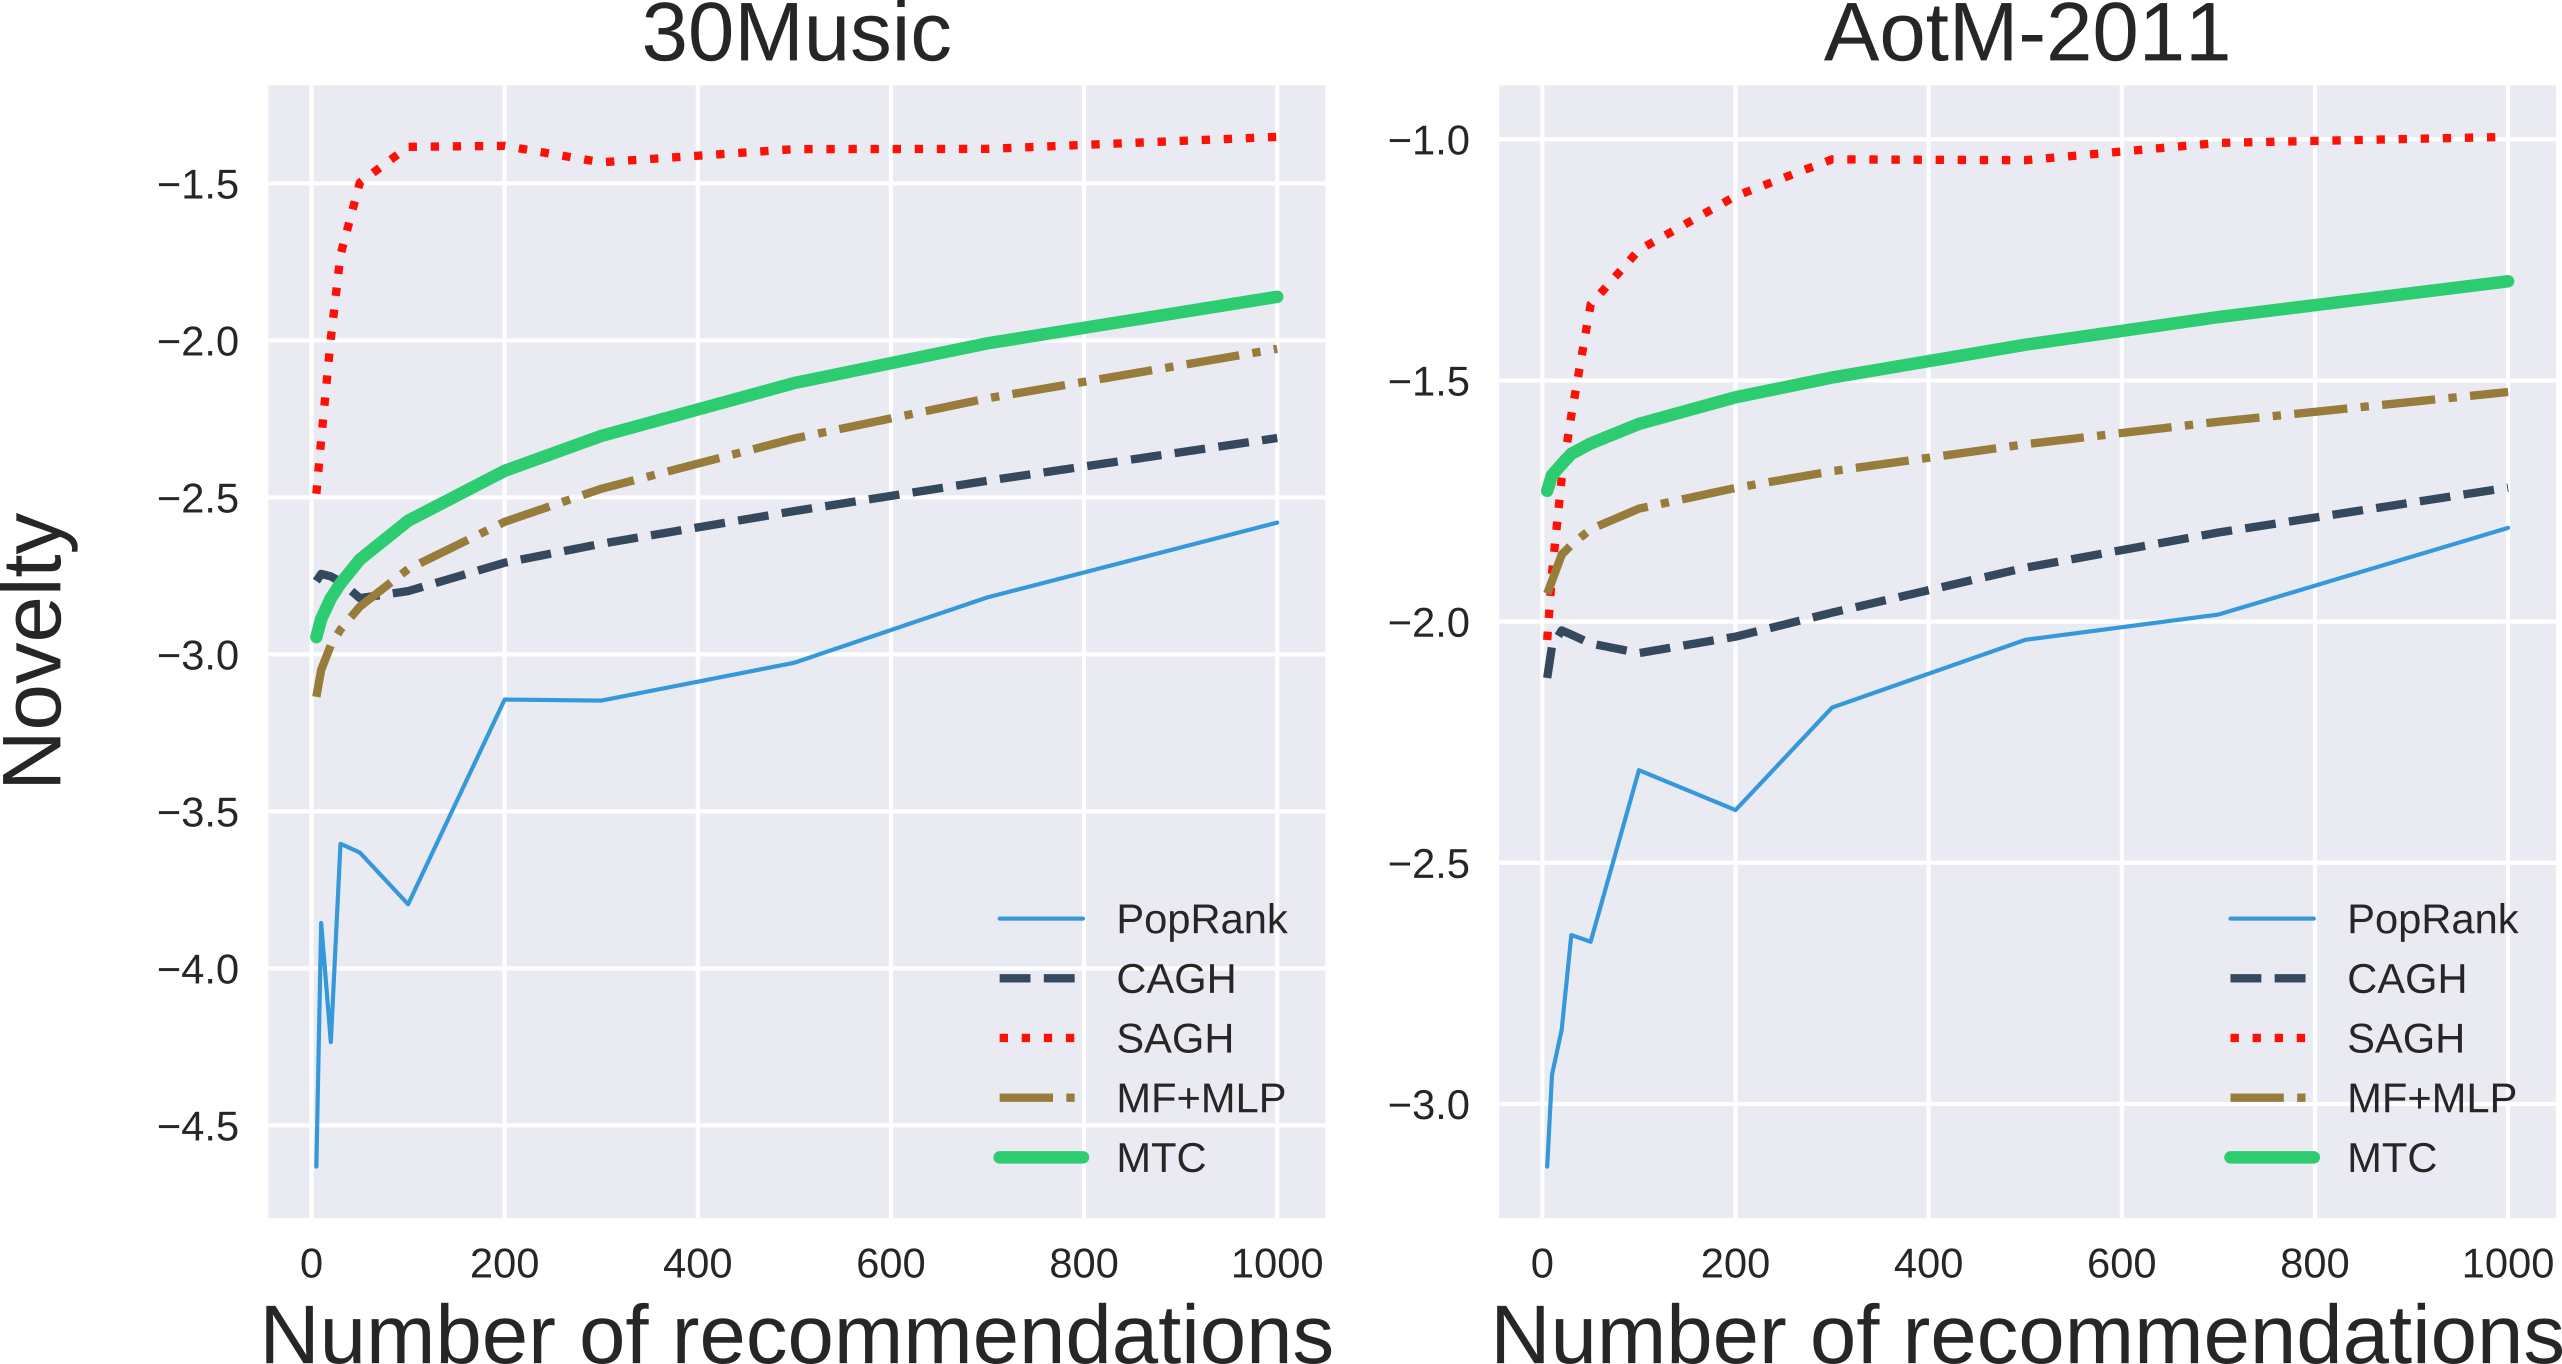
\includegraphics[width=\linewidth]{fig/nov1.png}
        \caption{Novelty for {\it cold songs}}
        \label{fig:nov1}
    \end{minipage}\hspace{11pt}%
    \begin{minipage}{0.32\textwidth}
        \centering
        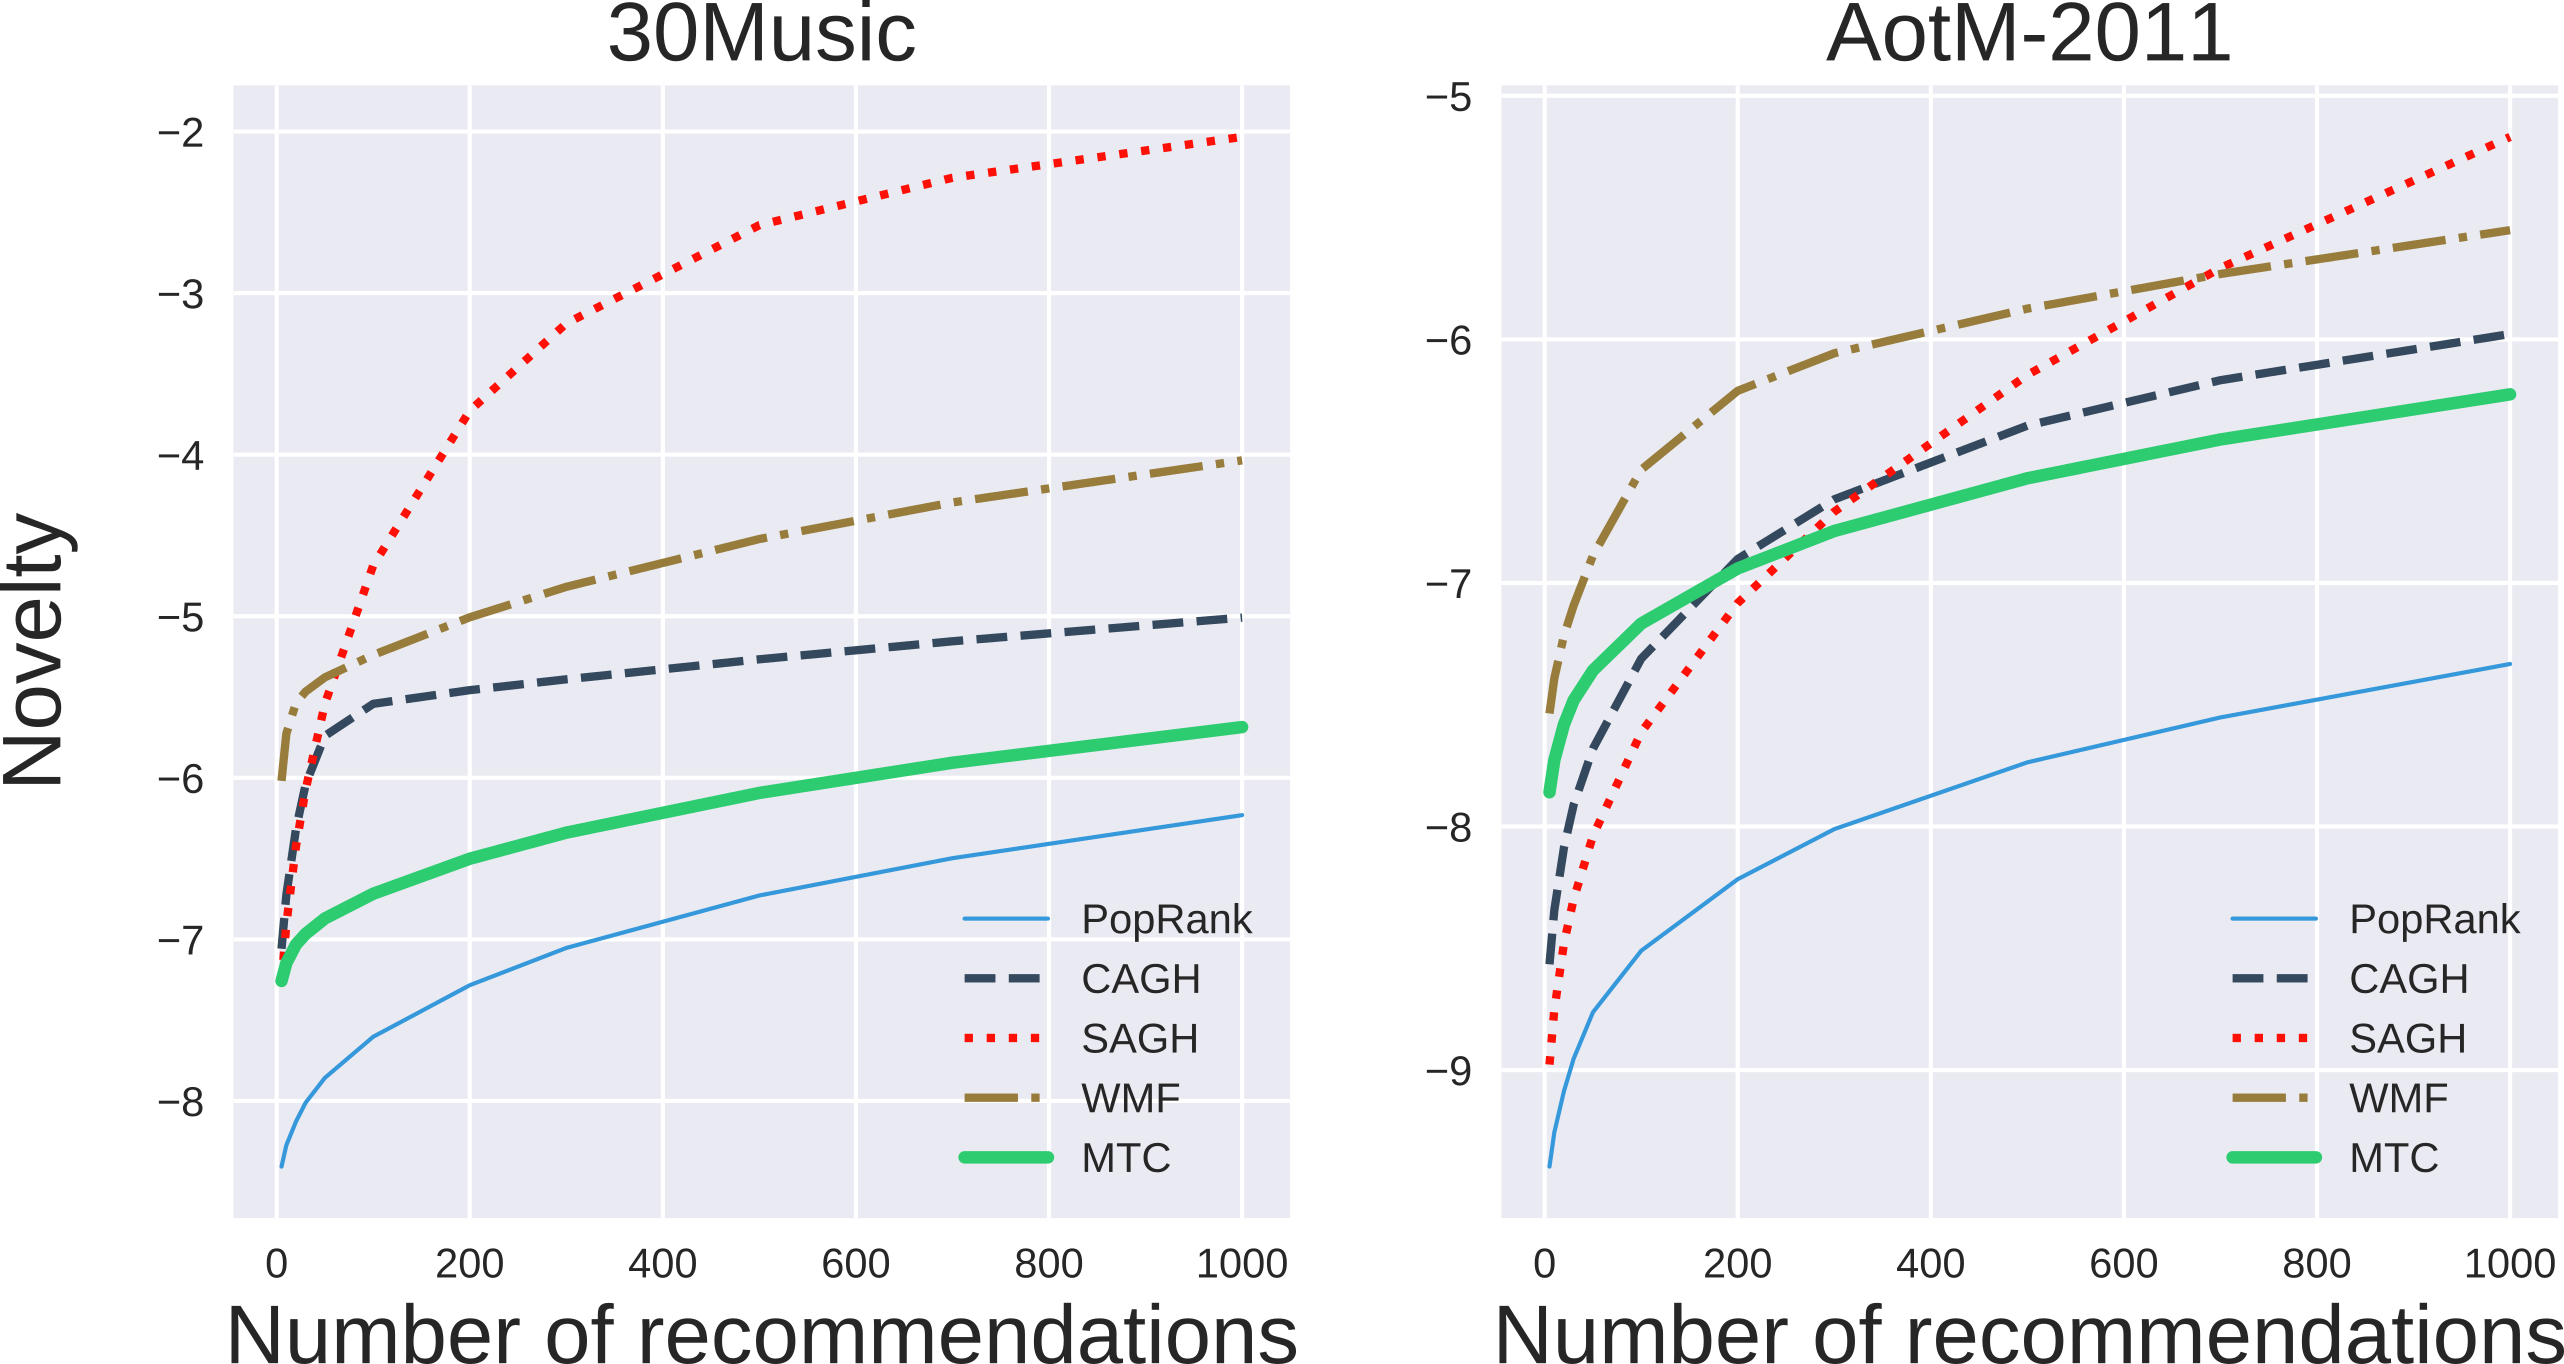
\includegraphics[width=.96\linewidth]{fig/nov3.png}
        \caption{Novelty for {\it cold playlists}}
        \label{fig:nov3}
    \end{minipage}\hspace{8pt}%
    \begin{minipage}{0.32\textwidth}
        \centering
        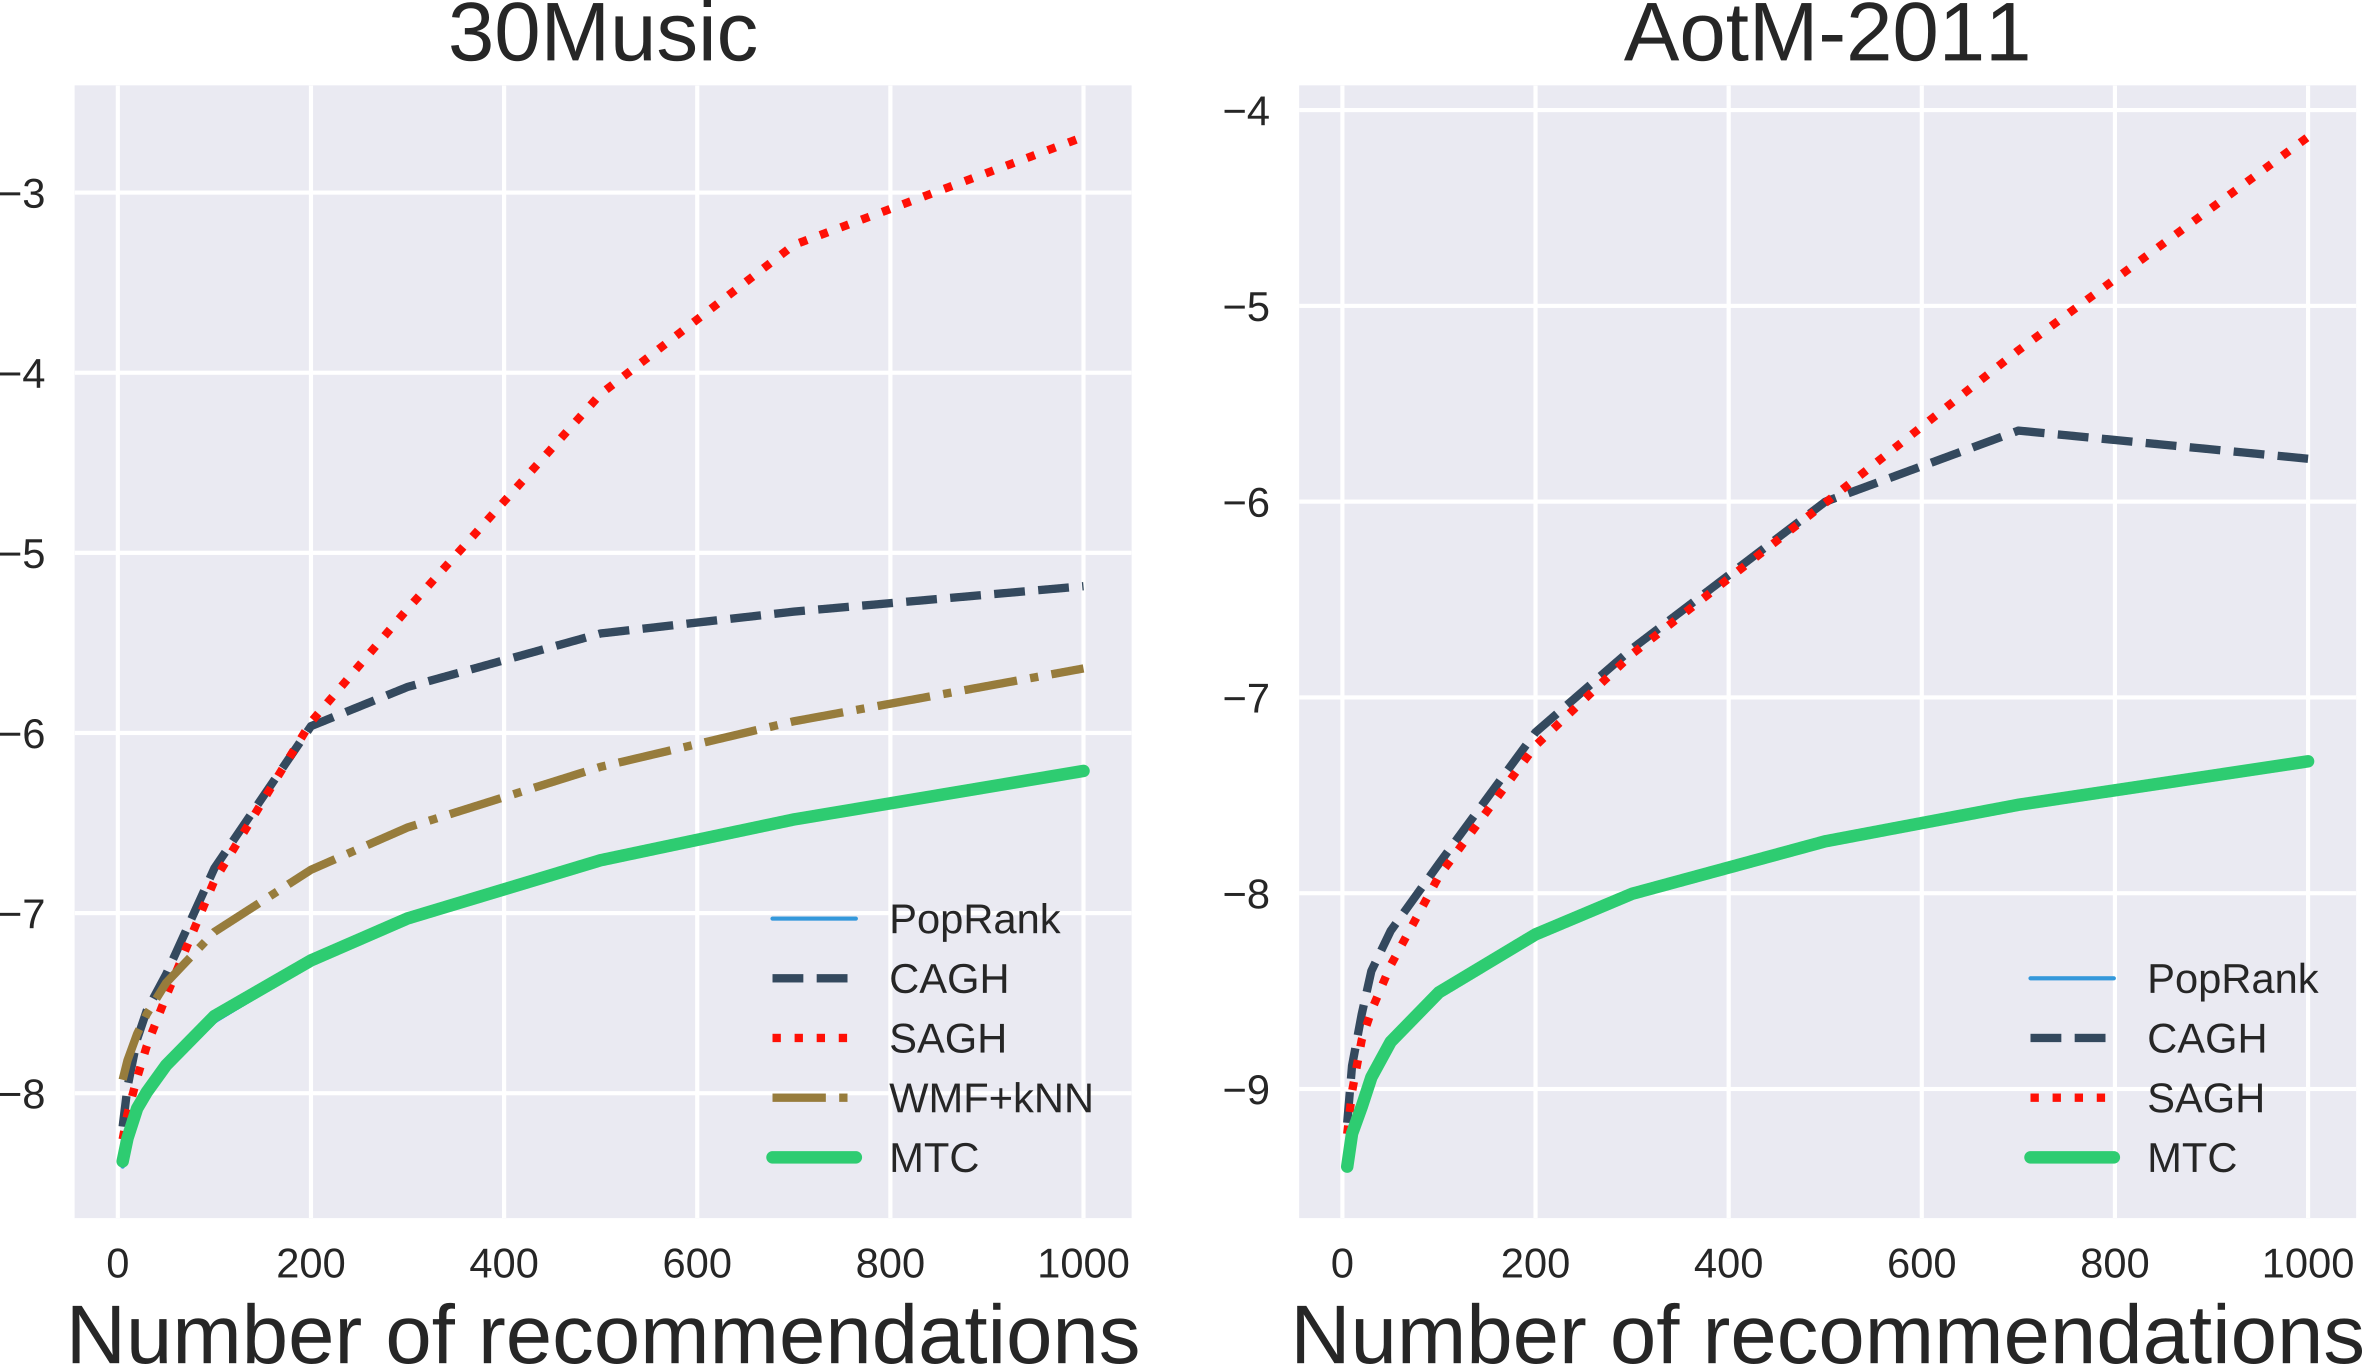
\includegraphics[width=.96\linewidth]{fig/nov4.png}
        \caption{Novelty for {\it cold users}}
        \label{fig:nov4}
    \end{minipage}
\end{figure*}


\subsubsection{Accuracy}

We can see from Table~\ref{tab:acc1} that learning based methods (\ie {\it Multitask classification}
and {\it Logistic Regression}) perform significantly better than other baselines in the \emph{cold songs} setting.
%in the setting of recommending new songs for extending playlists (setting (i)).
This suggests learning from playlists data helps the task of recommending new songs to extend existing playlist.
Among the (artist) popularity based approaches, 
simply ranking songs by its artist popularity achieves decent performance,
and taking into account artist collocation information does not always improve performance.
In particular, the SAGH method which considers only songs from artists in existing playlist
perform the worst in both datasets.
%is the worst performer in terms of HitRate@100 and AUC.

Figure~\ref{fig:hr1} shows the hit rates of all methods when the number of recommendations $K$ varies from 5 to 1000.
We can see that the performance of all methods improves as the number of recommendations increases,
and learning based methods always perform better than ranking approaches based on artist information.
It is interesting to observe that both {\it Multitask Classification} and {\it Logistic Regression} perform 
almost the same when $K$ is small (less 100 on 30Music and less 50 on AotM-2011 dataset), 
and the former only performs better when $K$ becomes bigger.
Another interesting observation is that SAGH and CAGH perform similarly on the AotM-2011 dataset when $K$
is less 50, and both outperform {\it Popularity Ranking}. However, SAGH suffers from slow improvement
as $K$ increases, and this effect is observed on both datasets.

Figure~\ref{fig:hr3} and Table~\ref{tab:acc3} show the performance of all methods in the \emph{cold playlists} setting.
%on the task of recommending a set of songs for an existing user (setting (ii)).
First, we can see that methods based on song popularity and artist information achieve good performance.
This is consistent with discoveries in~\cite{bonnin2013evaluating,jannach2015beyond,bonnin2015automated} which 
show ranking based on song popularity is a strong baseline.
Further, methods that make use of both song popularity and artist information
outperform {\it Popularity Ranking} (except SAGH on 30Music), which shows artist information is helpful for 
recommending music to form new playlists (for existing users).
This is in line with results reported in~\cite{bonnin2013evaluating,bonnin2015automated}.
%
%It is interesting to see that {\it Popularity Ranking}) perform worse than other methods in terms of HitRate@100,
%but SAGH performs worse than other methods in terms of AUC,
%which might suggest that SAGH achieves good recall but {\it Popularity Ranking} performs better on average.
It is interesting to observe that SAGH is one of the best performer on the AotM-2011 dataset (Figure~\ref{fig:hr3}), 
while it performs the worst in terms of HitRate@K on the 30Music dataset when $K$ is greater than 300.
%The performance of SAGH is also saturated much earlier than other methods.
%
%performance of all methods improves when $K$ increases, and {\it Multitask Classification}
%achieves the best performance on both datasets.
%However, while CAGH performs as good as {\it Multitask Classification} on 30Music,
%it is SAGH that achieves the best performance among all methods that ranks song by popularity and artist information
%on the AotM-2011 dataset, this might reflect the different characteristics between the two playlist dataset.


The performance in the \emph{cold users} setting %of recommending music to form playlists for new users (setting (iii)),
%however, 
is quite different from the other two cold-start settings, as shown in Figure~\ref{fig:hr4} and Table~\ref{tab:acc4}.
{\it Popularity Ranking} is one of the best performing methods,
outperforming both baselines that make use of song popularity and artist information (\ie SAGH and CAGH).
The performance of {\it Multitask Classification} is almost identical to that of {\it Popularity Ranking} in terms of both metrics,
which suggests {\it Multitask Classification} might degenerate to simply rank songs according to their popularity.
Another interesting observation is CAGH performs significantly better than SAGH,
% in terms of AUC and HitRate@K (when $K$ is greater than 100)
although both methods exploit song popularity as well as artist information.
This suggests the way to make use of artist information matters,
and collocation of artists could be more helpful than simply filtering out songs that are not from popular artists
when recommending music for new users.

Last but not the least, our proposed method {\it Multitask Classification}, unlike any other method in consideration,
is always the (tied) best performer in all three cold-start settings on both datasets.
This suggests our proposed approach can work effectively for the cold-start settings considered in this paper.

As a remark, the performance of all methods in terms of HitRate@K improves as the number of recommendations increases,
and the rate of improvement decreases as more songs are recommended.
In particular, the performance of SAGH tends to saturate much earlier than other methods 
(except in the \emph{cold playlists} setting on the AotM-2011 dataset),
which might suggest that, as more songs are recommended, artists in users' listening history (or popular artists) become less informative,
and other factors such as song popularity regain the dominance for the task of playlist recommendation in cold start settings.


\subsubsection{Novelty and spread}
% Unlike the accuracy metrics, where higher values indicate better performance,
% moderate values of Novelty and Spread are usually preferable~\cite{kluver2014evaluating,schedl2017}.
% While higher accuracy is usually preferred, 
% moderate values of novelty and spread are preferred~\cite{kluver2014evaluating,schedl2017}.
% moderate values are preferred.

\begin{table}[!t]
\caption{Spread for playlist recommendation in three cold-start settings, \emph{moderate} values are preferable.}
\label{tab:spread}
\resizebox{\columnwidth}{!}{
\setlength\tabcolsep{2pt}
\begin{tabular}{lcccclcccclcccc}
\toprule 
\multicolumn{3}{c}{Cold Playlists} &&& \multicolumn{3}{c}{Cold Users} &&& \multicolumn{3}{c}{Cold Songs} \\ 
\cmidrule{1-3} \cmidrule{6-8} \cmidrule{11-13}
Method & 30Music & AotM-2011 &&& Method & 30Music & AotM-2011 &&& Method & 30Music & AotM-2011 \\ 
\cmidrule{1-3} \cmidrule{6-8} \cmidrule{11-13}
%\midrule
PopRank & {\large\: 9.8} & {\large  10.5} \rule{0pt}{9pt} &&&  
PopRank & {\large\: 9.8} & {\large  10.5} \rule{0pt}{9pt} &&&  
PopRank & {\large   7.4} & {\large   7.8} \rule{0pt}{9pt} \\
%                                      
CAGH    & {\large\: 5.8} & {\large\: 2.3} \rule{0pt}{9pt} &&&  
CAGH    & {\large\: 4.2} & {\large\: 5.3} \rule{0pt}{9pt} &&&  
CAGH    & {\large   4.3} & {\large   4.6} \rule{0pt}{9pt} \\
%                                      
SAGH    & {\large  10.3} & {\large  10.4} \rule{0pt}{9pt} &&&  
SAGH    & {\large  10.0} & {\large  10.7} \rule{0pt}{9pt} &&&  
SAGH    & {\large   6.5} & {\large   5.9} \rule{0pt}{9pt} \\
%
WMF     & {\large  10.7} & {\large  11.6} \rule{0pt}{9pt} &&&  
WMF+kNN & {\large  10.7} & N/A            \rule{0pt}{9pt} &&&
MF+MLP  & {\large   8.5} & {\large   9.2} \rule{0pt}{9pt} \\
%
MTC     & {\large\: 9.4} & {\large  10.4} \rule{0pt}{9pt} &&&  
MTC     & {\large\: 9.9} & {\large  11.4} \rule{0pt}{9pt} &&&  
MTC     & {\large   7.9} & {\large   8.3} \rule{0pt}{9pt} \\
\bottomrule
\end{tabular}
}
\end{table}


From Figure~\ref{fig:nov1} we can see that PopRank achieves the lowest Novelty as expected from the definition of Novelty.
The Novelty of SAGH increases dramatically when the number of recommendations is larger than 30 or 50, the reason could be the average 
numbers of songs from an artist is around between 30 and 50 as shown in Table~\ref{tab:stats_pldata}, and SAGH simply recommends random
songs from artists that are not appeared in users' listening history.
All other methods achieve moderate Novelty and hence perform better for recommending new songs.
Similar observations can be obtained from Figure~\ref{fig:nov3} for the cold playlists recommendation.
However, there are two differences: (i) the Novelty of SAGH increases less dramatically due to the set of songs being considered are from
all artists of users' previous playlists; (ii) the proposed method MTC achieves lower Novelty (in general) than CAGH and WMF, which indicates
that MTC trends to prefer popular songs to form new playlists for existing users.
It is interesting to see that, the MTC and PopRank perform identically in the cold users setting~(Figure~\ref{fig:nov4}),
which provides more evidence that MTC degenerates to rank songs according to popularity.
CAGH and the hybrid of matrix factorisation and nearest neighbour method generally perform better (in terms of Novelty) for recommending 
playlists for new users.

We can see from Table~\ref{tab:spread} that both PopRank and MTC can similarly spread the attention across all possible songs in all three
cold-start settings. 
In the cold songs setting, CAGH and SAGH focus on songs from artists in users' listening history and similar artists, which explains 
the relative low spread values.
However, in the cold playlists and cold users settings, SAGH improves its attention spreading due to the set of songs it focuses on 
is significantly bigger (\ie songs from all artists in users' previous playlists and the top-10 most popular artists, respectively).
Surprisingly, CAGH remains focuses on a relatively small set of songs in both settings.
Lastly, the three variants of matrix factorisation method can generally spread the attention cross all possible songs comparably well.
